\chapter{Model Development}\label{ch:model_development}
One of the goals for this project was to research, design and compare different neural network topologies. 
Some of these were feed-forward, convolutional and recurrent.
Continuing, some neural networks were made deep, first by adding fully connected layers to the existing type feed-forward, CNN or RNN.
Different configurations were tested, some proving to be efficient for achieving designated goals, and some less so.
Subject to futher research, we found that recurrent neural networks work best for speech recognition.
Therefore  the following comparison will be based on different RNNs configurations.\\\\

\section{Neural Network Comparison}\label{sec:NNComparison}

In this chapter two models are developed based on the simple LSTM model from the silicon-valley-data-science RNN tutorial \cite{rubashkin2017}. Firstly these models (including "their simple LSTM model") will be trained and tested on a small data set with the numbers:\\\\
$\left\{zero, one, two, three, four, five, six, seven, eight, nine \right\}$,\\\\
the same data used in Chapter \ref{ch:machine_learning} for the parameter comparison. After that, the best performing model shall be picked for a more detailed discription (with code) and futher trainig with a bigger data set of the english language.\\\\
Before the comparison of the 3 models, lets take a look at their structure in the following diagrams.
As mentioned earlier the two models that were developed are based on the silicon-valley-data-science simple LSTM model. Their model consist of two LSTM layers as shown in the diagram below (Figure \ref{fig:simple_LSTM}).
\begin{figure}[H]
	\centering
	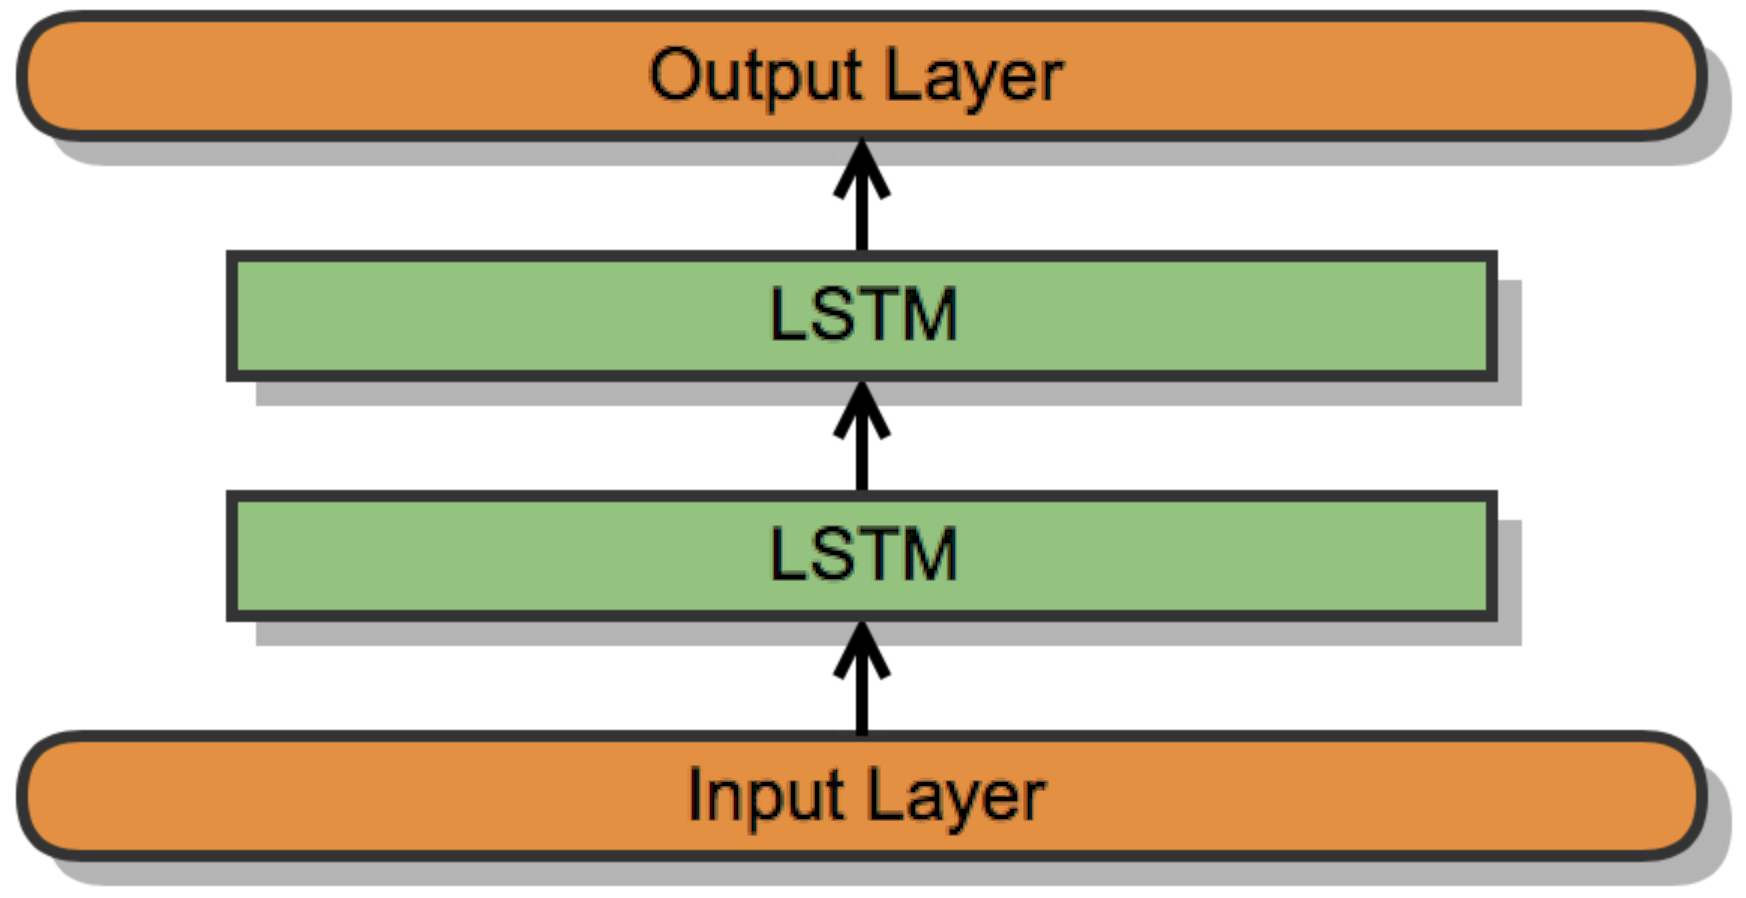
\includegraphics[width=.35\textwidth]		
	{model_development/01_simpleLSTM}
	\caption{Simple LSTM model.}
	\label{fig:simple_LSTM}
\end{figure}
Based on model above, it was decided among us to make an addition of two fully connected (FC) layers before and one FC layer after the two LSTM layers (shown in Figure \ref{fig:simple_LSTMFC}), with the desire of gaining better accuracy.
\begin{figure}[H]
	\centering
	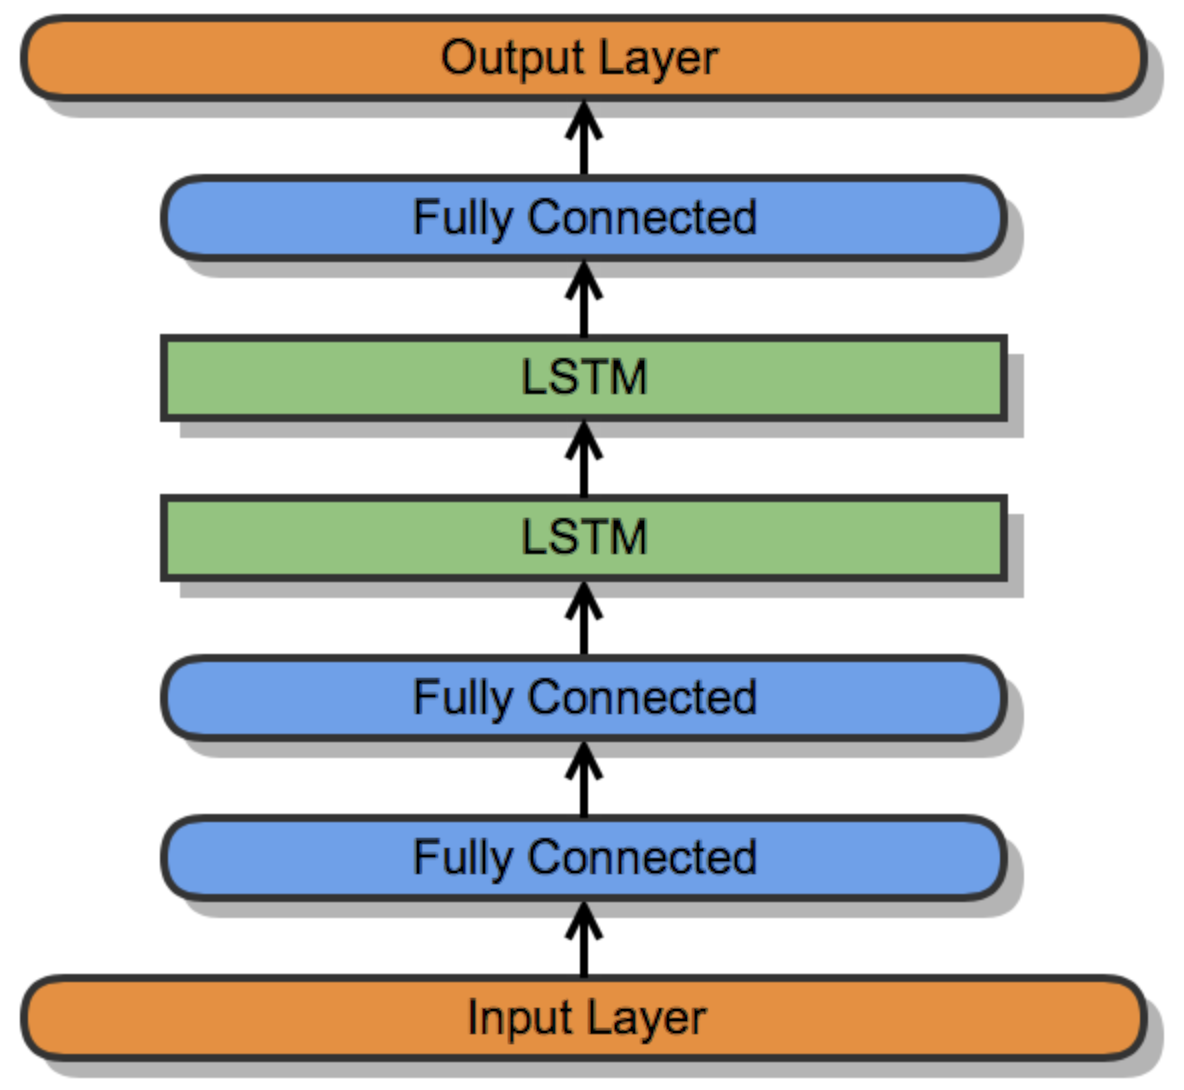
\includegraphics[width=.35\textwidth]		
	{model_development/02_simpleLSTMFC}
	\caption{Simple LSTM model with fully connected layers.}
	\label{fig:simple_LSTMFC}
\end{figure}
After that, a decision was made to replace the to LSTM layers in the model above with one Bi-Directional LSTM layers (seen in Figure \ref{fig:BiRNNFC}), again with the desire to make a more accurate model
\begin{figure}[H]
	\centering
	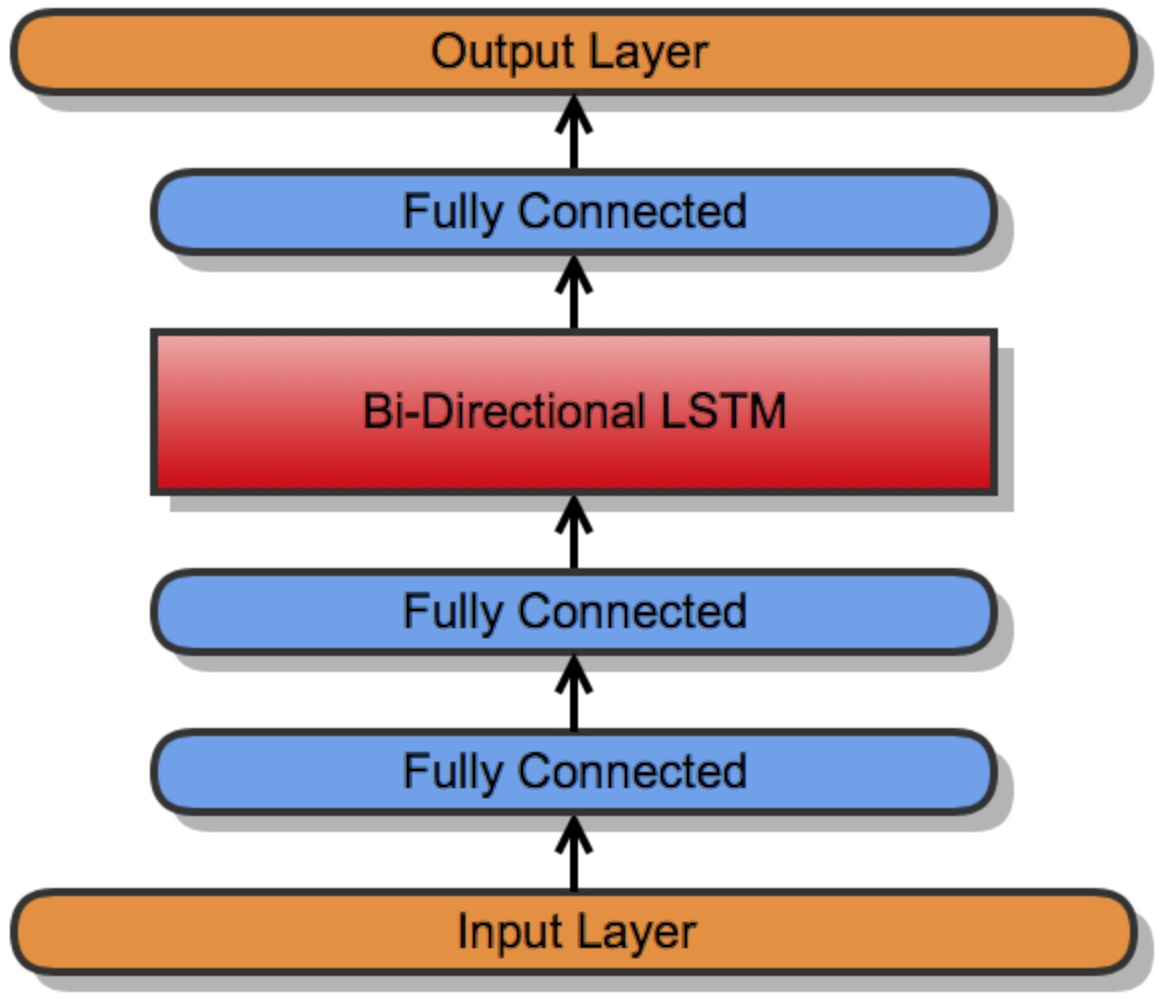
\includegraphics[width=.35\textwidth]		
	{model_development/03_BiRNN}
	\caption{BiRNN model with fully connnected layers.}
	\label{fig:BiRNNFC}
\end{figure}

In order to have a fair comparison between these model the paramaters values were made to be the same for all models as shown in Table \ref{tab:3models_tab}.
The respective models are mapped to the described ones in Table \ref{tab:3_models}. For the interested reader an expanded version in appendix \ref{ch:appClabel}.
\begin{table}[H]
\centering
    \caption{Parameter values of the three model.}
    \begin{tabular}{| l | c | c | c | c |} 
    \hline
        Parameters & 
        Model1 -\tikzcircle[pink, fill=pink]{3pt}- &
        Model2 -\tikzcircle[red, fill=red]{3pt}- &
        Model3 -\tikzcircle[turquoise, fill=turquoise]{3pt}-\\
    \hline
        Batch Size & 
        50 \hfill 20 \hfill 20 & 
        50 \hfill 20 \hfill 20 & 
        50 \hfill 20 \hfill 20 \\
    \hline
        Dropout & 
        0.05 & 0.05 & 0.05 \\
    \hline
        Learning Rate & 
        0.001 & 0.001 & 0.001 \\ 
    \hline
    \end{tabular}
    \label{tab:3models_tab}
\end{table}
\begin{table}[H]
\centering
	\caption{Models.}
	\begin{tabular}{ l  c }
	Model1 -\tikzcircle[pink, fill=pink]{3pt}- &
	(simple LSTM Model)\\
	Model2 -\tikzcircle[red, fill=red]{3pt}- &
	(simple LSTM + FC Model)\\
	Model3 -\tikzcircle[turquoise, fill=turquoise]{3pt}- &
	(BiRNN + FC Model)\\
	\end{tabular}
	\label{tab:3_models}
\end{table}

The following graph (Fig. \ref{fig:test_error_fig}) and
table (Tab. \ref{tab:test_error_tab}) represent the error
rate for the test data set. The results show that Model1 has $\sim 20\%$ word error rate (WER) while
Model2 and Model3 is $\sim 8\%$ and $\sim 0\%$ WER respectivly.

\begin{figure}[H]
	\centering
	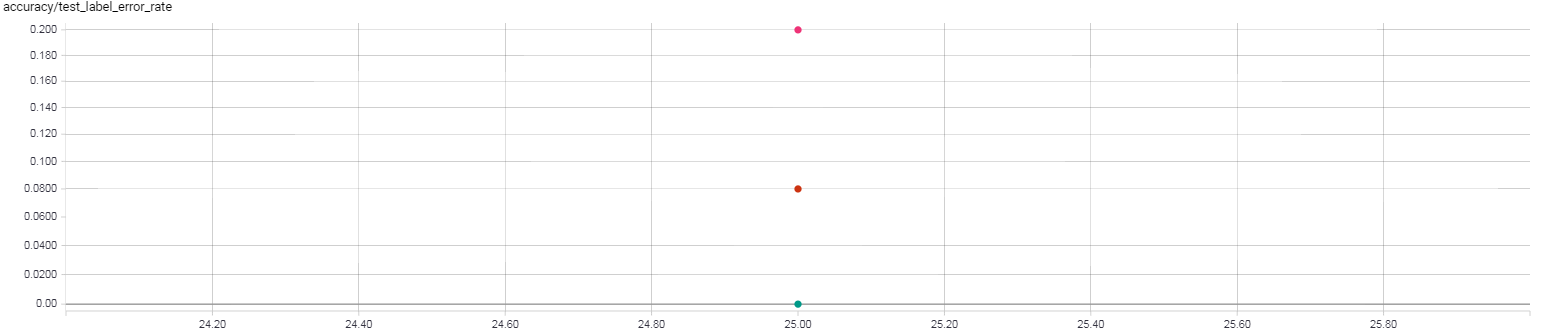
\includegraphics[width=\textwidth]		
	{model_development/3models_comparison/test_error_rate_3models}
	\caption{Test error rate.}
	\label{fig:test_error_fig}
\end{figure}

\begin{table}[H]
\centering
	\caption{Test error rate results.}
	\begin{tabular}{| l | c | c | c |}
	\hline
	Models & Value & Epoch & Duration \\
	\hline
	Model1 -\tikzcircle[pink, fill=pink]{3pt}- &
	0.200 & 25.00 & 0s\\
	\hline
	Model2 -\tikzcircle[red, fill=red]{3pt}- &
	0.080 & 25.00 & 0s\\
	\hline
	Model3 -\tikzcircle[turquoise, fill=turquoise]{3pt}- &
	0.000 & 25.00 & 0s\\
	\hline
	\end{tabular}
	\label{tab:test_error_tab}
\end{table}

The following graph (Fig. \ref{fig:validation_error_fig}) and
table (Tab. \ref{tab:validation_error_tab}) represent the error
rate for the validation data set. The results show that Model1 has took $\sim 7m 9s$ to complete training while
Model2 and Model3 is $\sim 9m 8s$ and $\sim 11m 49s$ respectivly.

\begin{figure}[H]
	\centering
	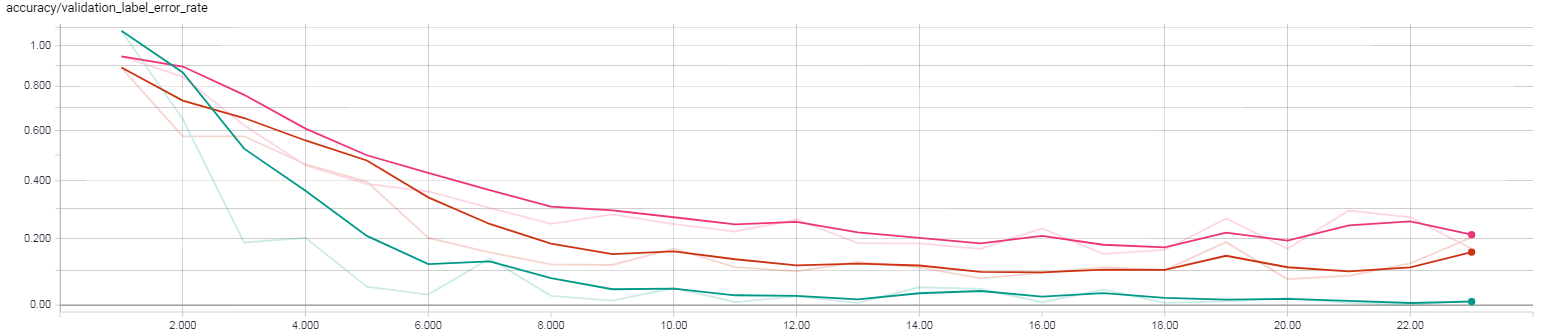
\includegraphics[width=\textwidth]		
	{model_development/3models_comparison/validation_error_rate_3models}
	\caption{Validation error rate.}
	\label{fig:validation_error_fig}
\end{figure}

\begin{table}[H]
\centering
	\caption{Validation error rate results.}
	\begin{tabular}{| l | c | c | c |}
	\hline
	Models & Value & Epoch & Duration \\
	\hline
	Model1 -\tikzcircle[pink, fill=pink]{3pt}- &
	0.1669 & 23.00 & 7m 9s\\
	\hline
	Model2 -\tikzcircle[red, fill=red]{3pt}- &
	0.2030 & 23.00 & 9m 8s\\
	\hline
	Model3 -\tikzcircle[turquoise, fill=turquoise]{3pt}- &
	0.01398 & 23.00 & 11m 49s\\
	\hline
	\end{tabular}
	\label{tab:validation_error_tab}
\end{table}

The final results show that Model1 was improved by adding the fully connected layers (Model2) from $\sim 20\%$ to $\sim 8\%$ WER and futher improved by adding the replacing the Bi-Directional LSTM layer (Model3) from $\sim 8\%$ to $\sim 0\%$ WER.
The graph for the validation error rate (Figure \ref{fig:validation_error_fig}) clearly shows the three distict lines in "parallel" with each other. The top line being the least accurate and the bottom one being the most.

\section{Model Description}

Model3 (BiRNN) is better therefore we go into more detail about it...

\todo{Make full page png}
\begin{figure}[H]
	\centering
	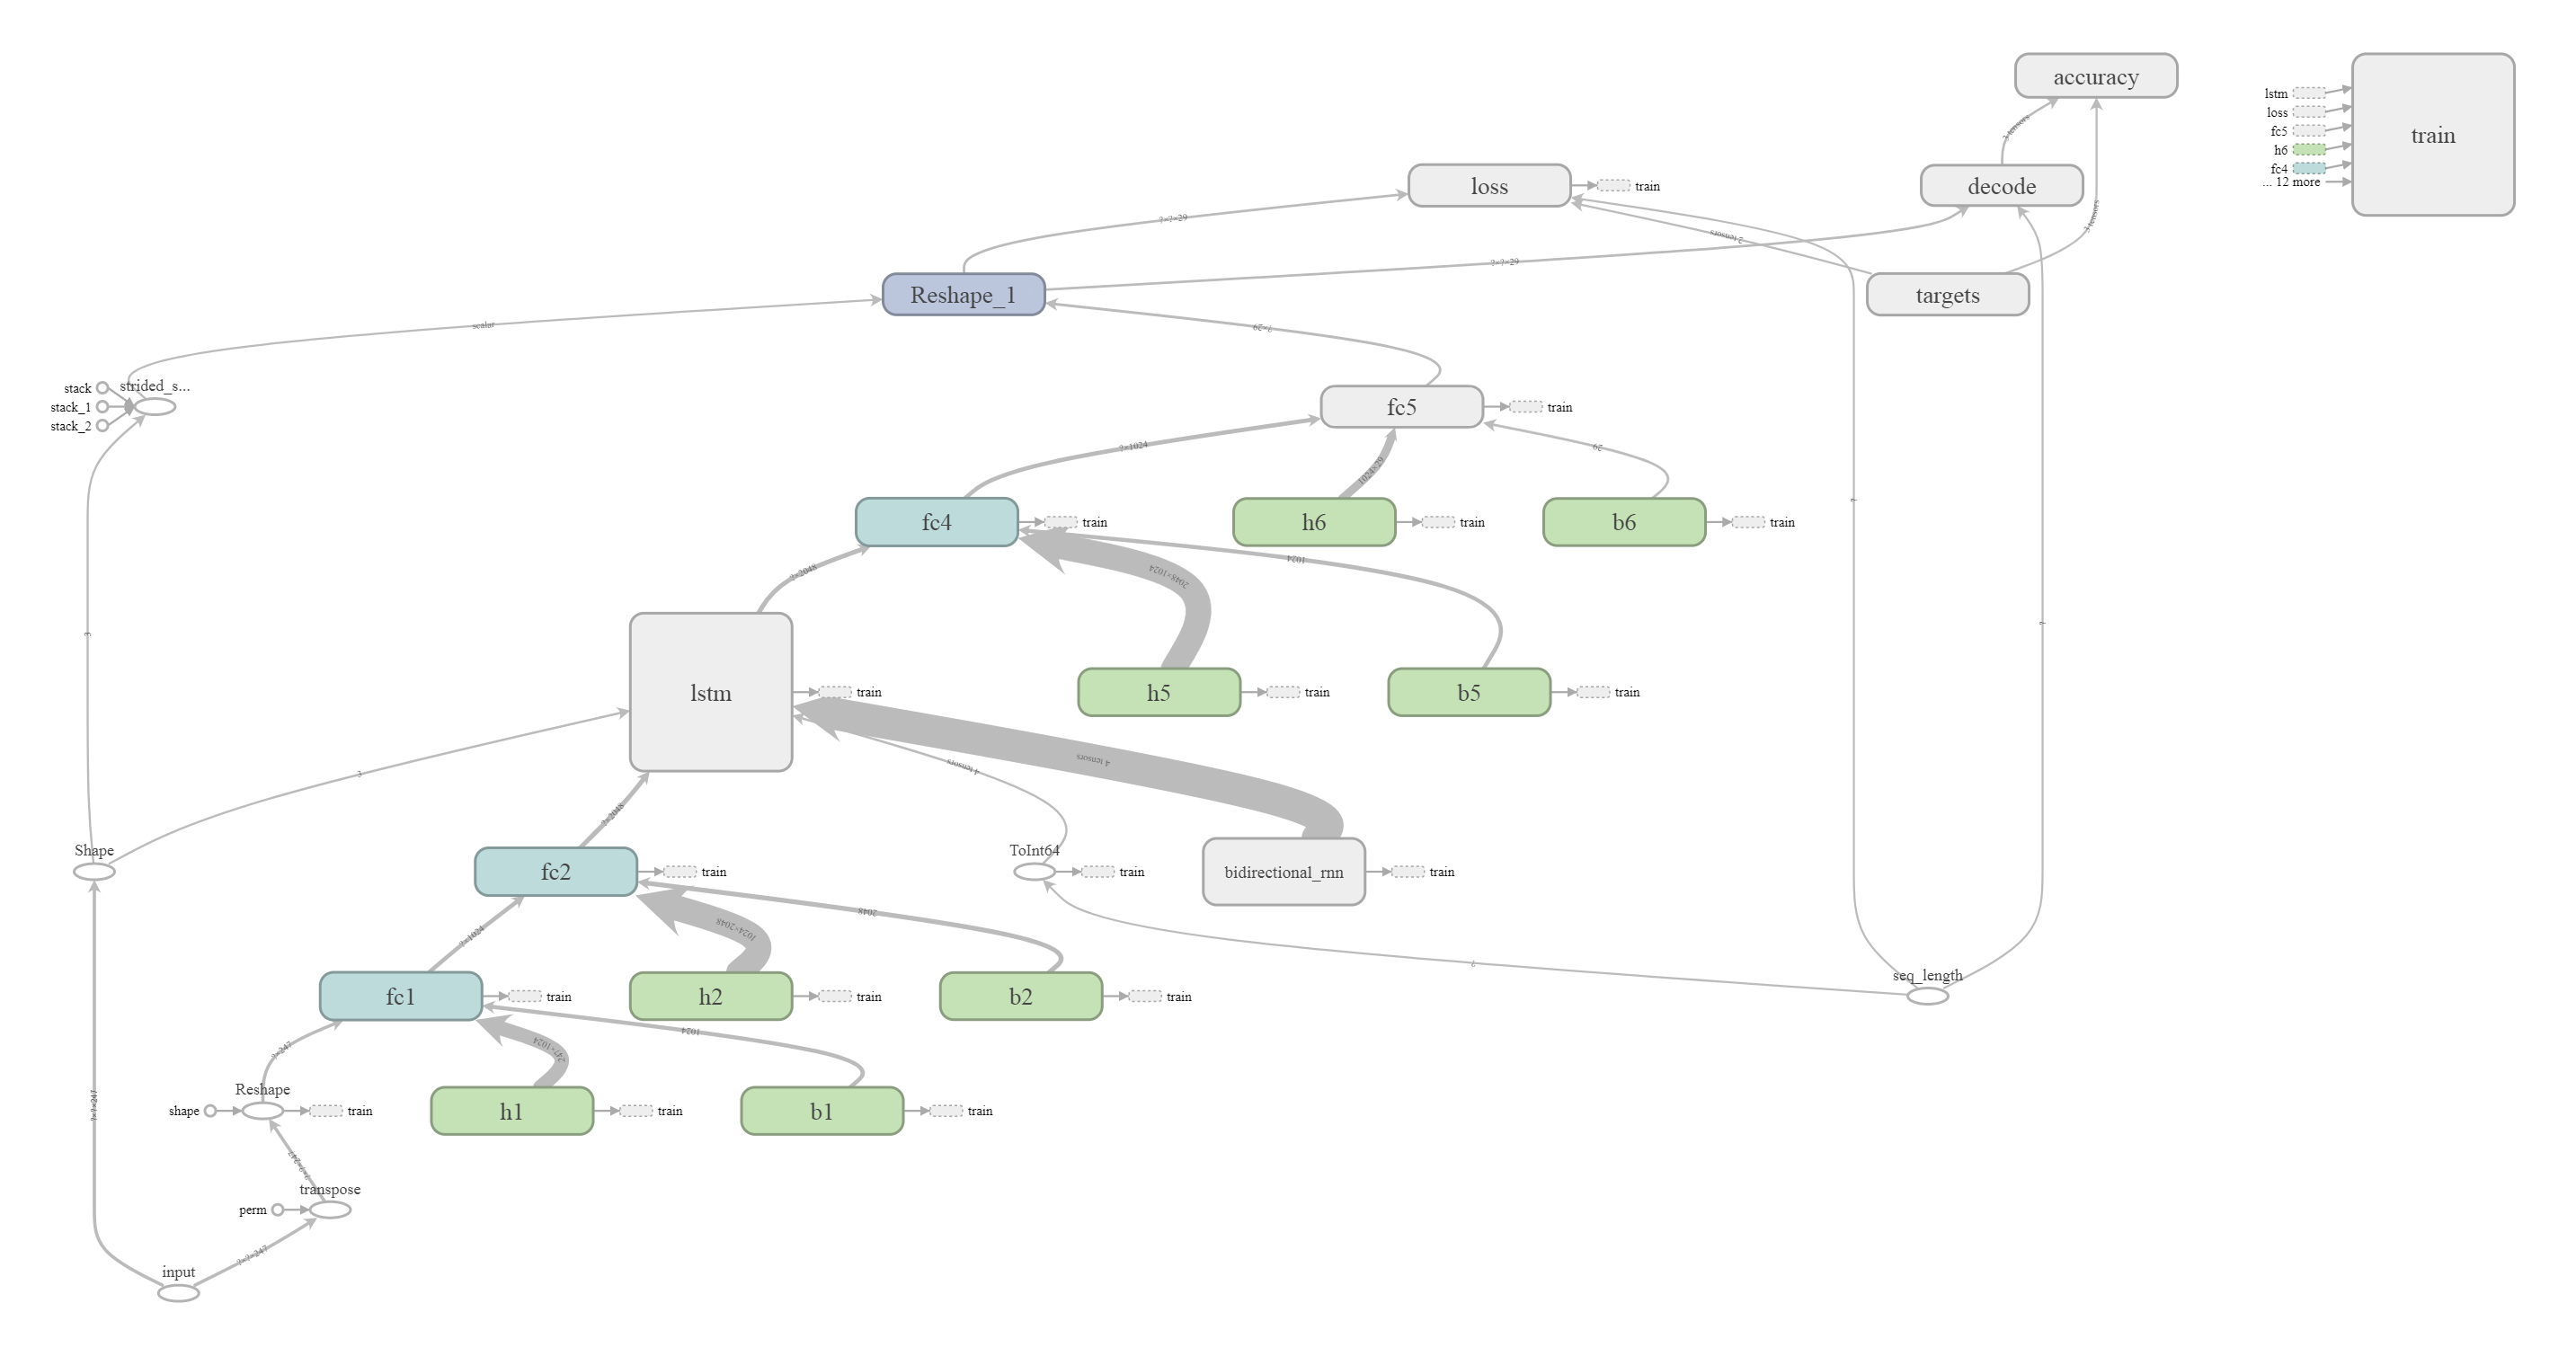
\includegraphics[width=\textwidth]		
	{model_development/birnn_v2_graph}
	\caption{Our BiRNN model graph.}
\end{figure}

As shown in a previous chapter,\todo{reference which chapter we talk about} the model that is used in this DSR system is a recurrent neural network.

This recurrent network is based on the standard LSTM cell, but used as a bidirectional layer. 
The purpose is to recognize the context of the text, to improve the prediction. 
The complete topology for the network is as follows: \\\\
\todo{INSERT NICE PICTURE DESCRIPTION HERE} \\\\
Described in figure X is the complete topology of the network used in the current implementation. It has a structure of 2-BiRNN-1-logits. In the beginning it has 2 fully connected layers, each consisting of 1024 neurons.

\lstinputlisting[language=Python, firstline=36, lastline=51]{code/txtFileMaker.py}

Further on, the input is reshaped to be compatible with the BiRNN layer, consisting of two LSTM cells, each with 1024 neurons.
One cell is used in the "forward" direction, and the other one in the "backward" direction, with the goal of understanding the current context.
Following this step, the input is reshaped again and sent to the next fully connected layer.
The final layer, the logits layer, is used as output of the network. At this point, the original input is transformed by every layer and sent for decoding.
\todo{add caption}
\todo{clarify types of nn}

